\small
%\section{材料电子结构计算软件的基本结构}       %Bookmark
%\frame
%{
%	\frametitle{科学研究的范式变更}
%\begin{figure}[h!]
%\vspace*{-0.18in}
%\centering
%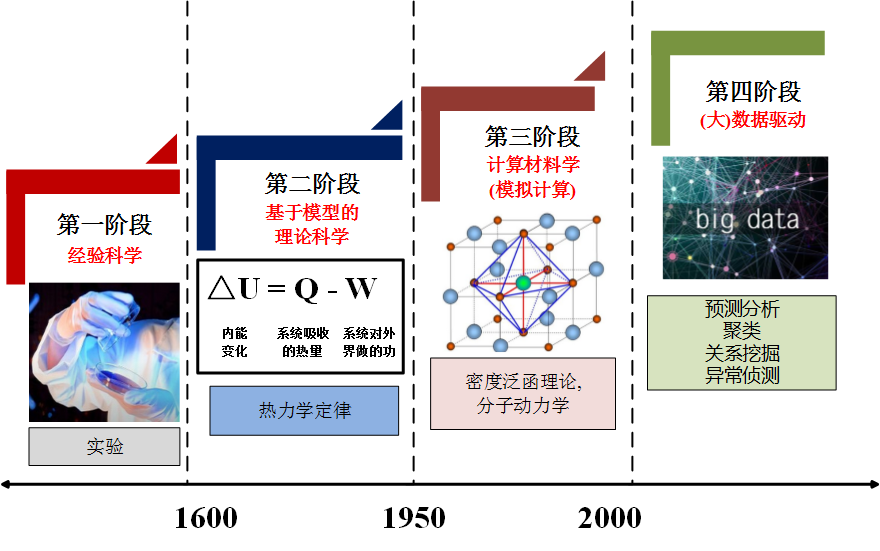
\includegraphics[width=4.05in]{Figures/Four_Model.png}
%%\caption{\tiny \textrm{Pseudopotential for metallic sodium, based on the empty core model and screened by the Thomas-Fermi dielectric function.}}%(与文献\cite{EPJB33-47_2003}图1对比)
%\label{Four_Model}
%\end{figure}
%}
%
\frame
{
	\frametitle{材料基因工程的基本思想}
\begin{figure}[h!]
\centering
\vspace*{-0.2in}
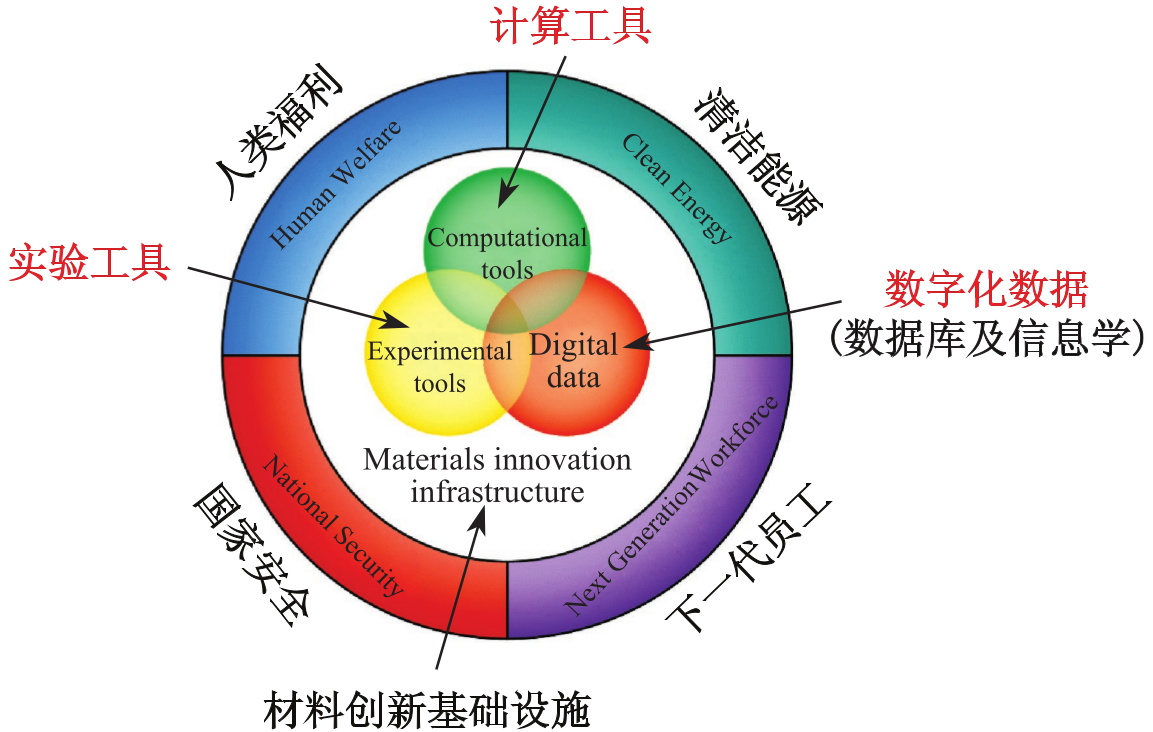
\includegraphics[width=0.6\textwidth]{Figures/Mat_Geno_Ene-1.png}
\vskip 0.10in
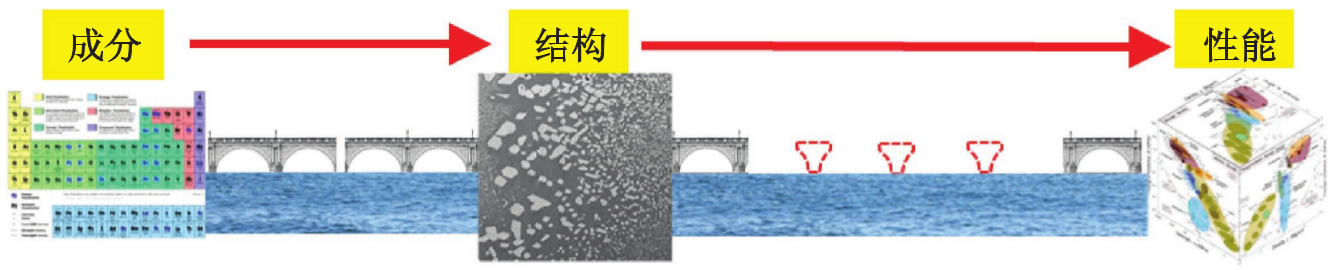
\includegraphics[height=0.85in]{Figures/Mat_Geno_Ene-3.png}
\label{Mater_Genome}
\end{figure}
}

%\section{高通量材料计算平台开发现状}     %Bookmark
%\frame
%{
%	\frametitle{现有高通量计算平台概览}
%\begin{table}[!h]
%\tabcolsep 0pt \vspace*{-12pt}
%%\caption{}
%\label{Table-Cost}
%\begin{minipage}{0.85\textwidth}
%%\begin{center}
%\centering
%\def\temptablewidth{1.1\textwidth}
%\renewcommand\arraystretch{0.8} %表格宽度控制(普通表格宽度的两倍)
%\rule{\temptablewidth}{1pt}
%\begin{tabular*} {\temptablewidth}{@{\extracolsep{\fill}}c@{\extracolsep{\fill}}c@{\extracolsep{\fill}}c@{\extracolsep{\fill}}c@{\extracolsep{\fill}}c@{\extracolsep{\fill}}c@{\extracolsep{\fill}}c}
%%-------------------------------------------------------------------------------------------------------------------------
%	&\multirow{2}{*}{\fontsize{7.2pt}{5.2pt}\selectfont{编程语言}}	&\fontsize{7.2pt}{5.2pt}\selectfont{建模} &\multicolumn{2}{|c|}{\fontsize{6.2pt}{5.2pt}\selectfont{任务提交与管理}} &\multirow{2}{*}{\fontsize{7.2pt}{5.2pt}\selectfont{后处理}} &\multirow{2}{*}{\fontsize{6.2pt}{5.2pt}\selectfont{数据组织管理}} \\\cline{4-5}
%	&	&\fontsize{7.2pt}{5.2pt}\selectfont{功能} &\multicolumn{1}{|l}{\fontsize{7.2pt}{5.2pt}\selectfont{软件接口}} &\multicolumn{1}{r|}{\fontsize{7.2pt}{5.2pt}\selectfont{运行容错}} & & \\\hline
%	\fontsize{7.2pt}{5.2pt}\selectfont{{AFLOW}} &\fontsize{7.2pt}{5.2pt}\selectfont{C++} &\checkmark &\triangle &\FiveStarOpen &\FiveStarOpen &\fontsize{7.2pt}{5.2pt}\selectfont{{Django}} \\
%	\fontsize{7.2pt}{5.2pt}\selectfont{{MP}} &\fontsize{7.2pt}{5.2pt}\selectfont{Python} &\checkmark &\checkmark &\FiveStarOpen &\FiveStarOpen &\fontsize{7.2pt}{5.2pt}\selectfont{{MongoDB}} \\
%	\multirow{2}{*}{\fontsize{7.2pt}{5.2pt}\selectfont{{QMIP}}} &\fontsize{7.2pt}{5.2pt}\selectfont{JavaScript/SVG} &\multirow{2}{*}{\checkmark} &\multirow{2}{*}{\checkmark} &\multirow{2}{*}{--} &\multirow{2}{*}{\checkmark} &\multirow{2}{*}{--} \\
%	&\fontsize{7.2pt}{5.2pt}\selectfont{+html/Python} & & & & & \\
%	\fontsize{7.2pt}{5.2pt}\selectfont{{CEP}} &\fontsize{7.2pt}{5.2pt}\selectfont{Python} &\checkmark &\checkmark &-- &\checkmark &\fontsize{7.2pt}{5.2pt}\selectfont{{Django/MySQL}} \\
%	\fontsize{7.2pt}{5.2pt}\selectfont{{ASE}} &\fontsize{7.2pt}{5.2pt}\selectfont{Python} &\FiveStarOpen &\FiveStarOpen &-- &\triangle &-- \\
%	\multirow{2}{*}{\fontsize{7.2pt}{5.2pt}\selectfont{{MatCloud}}} &\fontsize{7.2pt}{5.2pt}\selectfont{JavaScript} &\multirow{2}{*}{\checkmark} &\multirow{2}{*}{\triangle} &\multirow{2}{*}{\checkmark} &\multirow{2}{*}{\checkmark} &\multirow{2}{*}{\fontsize{7.2pt}{5.2pt}\selectfont{{MongoDB}}} \\
%	&\fontsize{7.2pt}{5.2pt}\selectfont{+.NETCore} & & & & &
%\end{tabular*}
%\rule{\temptablewidth}{1pt}
%\end{minipage}
%%\vskip -15pt
%\fontsize{7.2pt}{5.2pt}\selectfont{
%\begin{description}
%	\item[\FiveStarOpen]~该功能较突出
%	\item[\checkmark]~该功能基本满足需求
%	\item[\triangle]~该功能存在不足
%\end{description}}
%%\end{center}
%\end{table}
%\fontsize{8.2pt}{6.2pt}\selectfont{
%	\textrm{Lin L. \textit{Materials databases infrastructure constructed by first principles calculations:~a review.} \textbf{Mater. Perform. Character.}, 2015, 4(1):148.}}
%}
%
\section{自主材料设计流程一体机}     %Bookmark

\frame
{
	\frametitle{\textrm{计算平台的功能和总体架构}}
\begin{figure}[h!]
\centering
\vspace*{-0.35in}
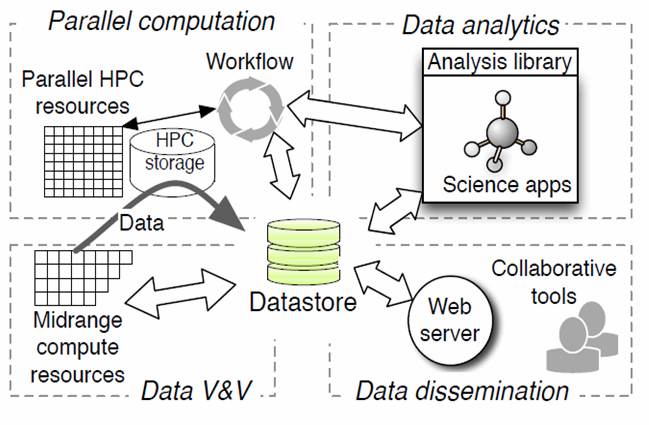
\includegraphics[height=2.6in,width=4.05in,viewport=0 0 670 460,clip]{Figures/Parallel_computation.png}
%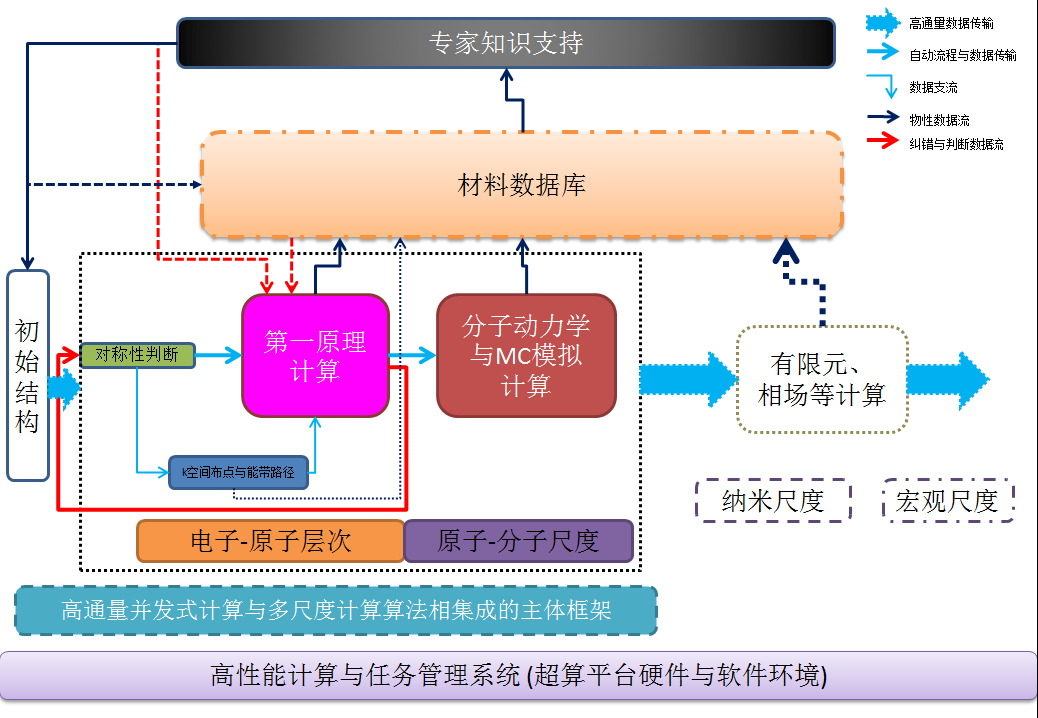
\includegraphics[height=1.6in,width=2.4in,viewport=0 0 1038 730,clip]{Figures/Auto_Flow.png}
\caption{\fontsize{7.2pt}{4.2pt}\selectfont{\textrm{The schematic framework and platform of all those project.}}}%
\label{Auto_Flow}
\end{figure} 
}

%\frame
%{
%	\frametitle{\textrm{MP}自动流程的设计与开发}
%	\begin{itemize}
%		\item \textcolor{red}{设计目标}:~围绕\textrm{VASP~}作业高通量并发提交与过程监控
%		\item \textcolor{red}{设计方案}:~开发针对不同计算场景的功能模块
%			\begin{enumerate}
%    \setlength{\itemsep}{15pt}
%				\item \textcolor{blue}{\textbf{Pymatgen}}\\
%					\textcolor{magenta}{前处理}:~计算模型的分析与预处理\\
%					\textcolor{magenta}{后处理}:~计算结果的可视化
%				\item \textcolor{blue}{\textbf{FireWorks}}\\
%\textcolor{magenta}{计算流程设计与管理}:~数据库支持的计算流程管理
%				\item \textcolor{blue}{\textbf{Custodian}}\\
%\textcolor{magenta}{计算流程容错与应对}:~提供计算过程错误判断接口,由用户提供解决策略和针对性设计
%			\end{enumerate}
%	\end{itemize}
%		%\item 计算过程的控制方式
%}
%
%\frame
%{
%	\frametitle{\textrm{Pymatgen}的模块结构}
%\begin{figure}[h!]
%\centering
%\vspace*{-0.1in}
%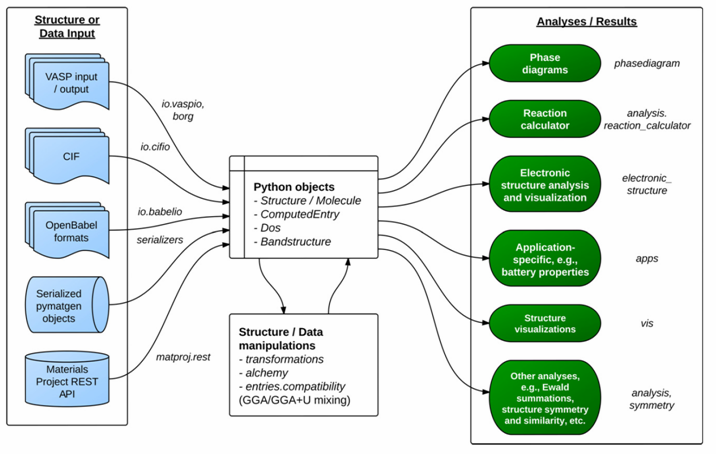
\includegraphics[height=2.3in]{Figures/MP_library.png}
%\caption{\fontsize{7.2pt}{4.2pt}\selectfont{\textrm{Overview of a typical workflow for pymatgen.}}}%
%\label{Pymatgen_Lib}
%\end{figure} 
%}
%
%\frame
%{
%	\frametitle{\textrm{Pymatgen}可展示的材料物性}
%\begin{figure}[h!]
%\centering
%\vspace*{-0.1in}
%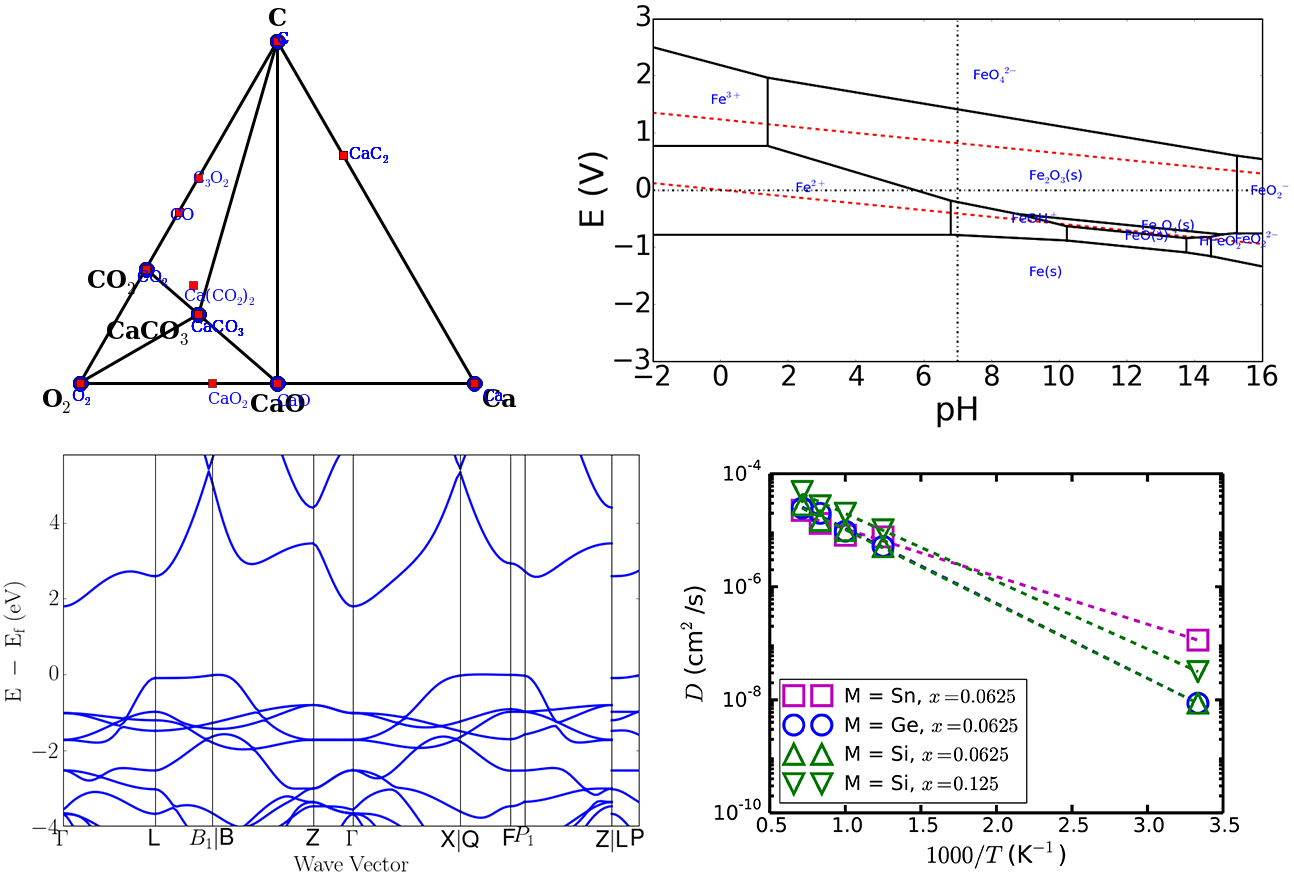
\includegraphics[height=2.3in]{Figures/MP_vision.png}
%\caption{\fontsize{5.2pt}{4.2pt}\selectfont{\textrm{Top left: Phase; Top right: Pourbaix diagram from the Materials API. \\Bottom left: Calculated bandstructure plot using pymatgen’s parsing and plotting utilities. Bottom right: Arrhenius plot using pymatgen’s Diffusion~Analyzer.}}}%
%\label{Pymatgen_vision}
%\end{figure} 
%}
%
%\frame
%{
%	\frametitle{\textrm{FireWorks}的模块结构}
%\textrm{FireWorks}发布的工作流成由三层嵌套结构组成:
%\fontsize{8.2pt}{6.2pt}\selectfont{
%\begin{itemize}
%	\item \textrm{Firetask}:~基本执行单元,是执行计算的最基本脚本命令或\textrm{Python}命令。
%	\item \textrm{Firework}:~组织基本执行单元构成任务单元组,并指定各基本执行单元所需的参数。
%	\item \textrm{Workflow}:~彼此相关联的任务单元组构成完整的工作流程:\\
%		\textrm{FireWork}之间的数据传递、任务执行序列等由\textrm{FWAction}完成。
%\end{itemize}}
%\begin{figure}[h!]
%\centering
%\vspace*{-0.1in}
%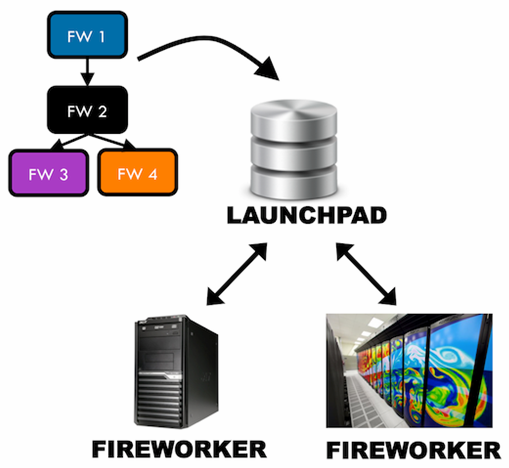
\includegraphics[height=1.5in]{Figures/MP_fireworks.png}
%\hskip 1pt
%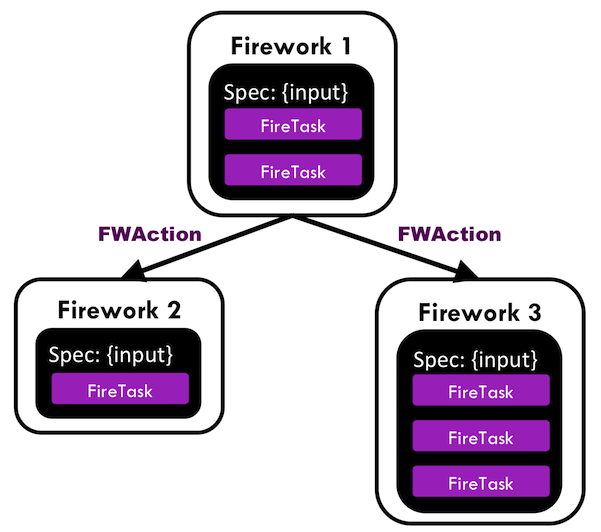
\includegraphics[height=1.5in]{Figures/MP_multiple_fw.png}
%\caption{\fontsize{7.2pt}{4.2pt}\selectfont{\textrm{The basic infrastructure of FireWorks.}}}%
%\label{FireWorks_FW}
%\end{figure} 
%}
%
%\frame
%{
%	\frametitle{\textrm{FireWorks}的模块结构}
%\fontsize{8.2pt}{6.2pt}\selectfont{
%	\begin{itemize}
%		\item \textrm{FireWorks}是以任务单元组为基本组成的来实现工作流程的,任务单元组之间依靠数据传递相关联,流程执行完毕也将返回数据,\textrm{FWAction}模块主要负责任务单元组之间的数据传递和任务分配。
%		\item \textrm{FWAction}允许用户根据需要设计和更改流程参数、增添、删减和改变流程(子)单元组,这一模块大大增加了\textrm{FireWorks}工作流的灵活性。}
%	\end{itemize}
%\begin{figure}[h!]
%\centering
%\vspace*{-0.15in}
%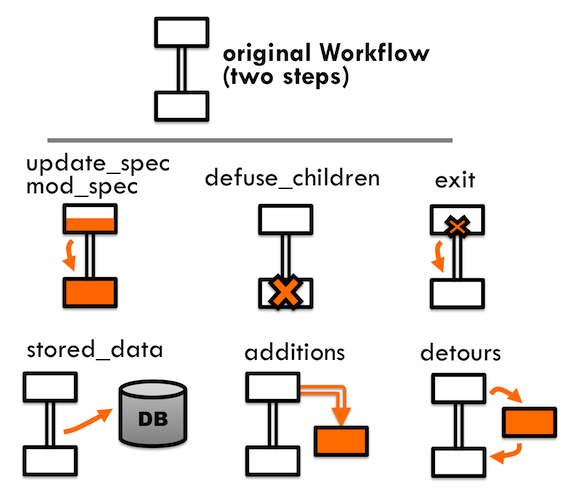
\includegraphics[height=1.9in]{Figures/MP_Fireworks_fwactions.png}
%\caption{\fontsize{7.2pt}{4.2pt}\selectfont{\textrm{FireWorks}的单元组间数据传递与处理示意.}}%
%\label{FireWorks_FWA}
%\end{figure} 
%}
%
%\frame
%{
%	\frametitle{\textrm{FireWorks}的模块结构}
%这种“发布-执行”结构使得计算任务与软件、硬件高度解耦,用户可根据需要随时向\textrm{LaunchPad}添加新的工作流,承担计算任务的\textrm{FireWorkers}彼此也可以是完全异构的,具有很好的机动性。
%\vskip 0.25in
%对于材料第一原理计算自动流程而言,一个\textrm{DFT}计算过程就是一个\textrm{Firework},可以分解为:
%\begin{enumerate}
%	\item 指定计算控制参数(参数在数据库中\texttt{Json}存储,由\textrm{Spec}传入)
%	\item 计算控制文件生成(每个\textrm{Firetask}生成一个控制文件)
%	\item \textrm{DFT}计算作业提交(一个\textrm{Firetask})
%\end{enumerate}
%在此基础上,可以通过\textrm{FWAction}修改控制参数,将\textrm{DFT}计算单元组组织成完整的材料第一原理计算流程,并将最终结果直接导入材料计算数据库。
%}

\frame
{
	\frametitle{\textrm{Custodian}的容错逻辑}
\begin{figure}[h!]
\centering
\vspace*{-0.1in}
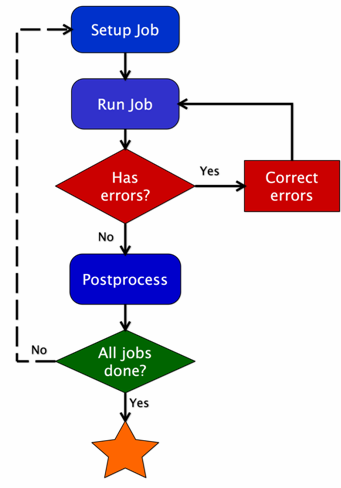
\includegraphics[height=2.3in]{Figures/MP_custodian.png}
\label{Custodian_over}
\caption{\fontsize{7.2pt}{4.2pt}\selectfont{\textrm{Overview of the Custodian workflow.}}}%
\end{figure} 
}

\frame
{
	\frametitle{\textrm{atomate}:~计算流程控制示范}
%		\textcolor{purple}{\textrm{Atomate}}:~:~适合一定复杂程度的\textrm{~VASP~}计算
\begin{figure}[h!]
\centering
\vspace*{-0.19in}
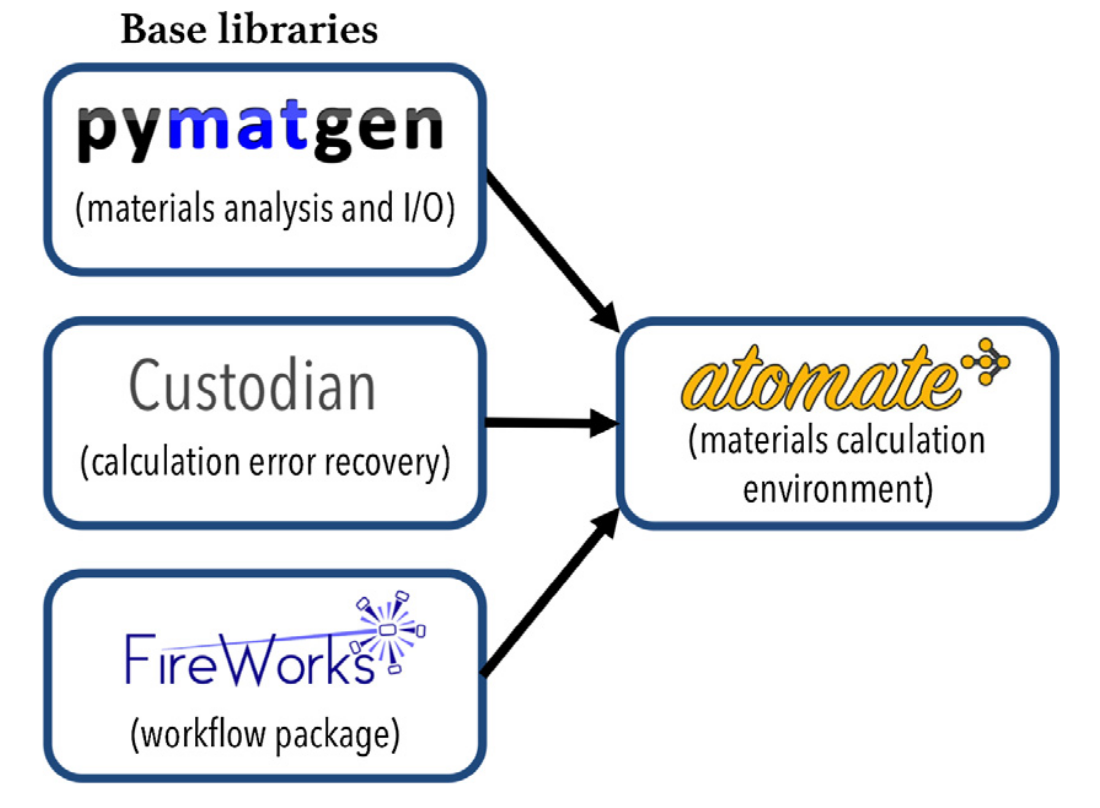
\includegraphics[height=1.4in,width=2.2in,viewport=0 0 820 630,clip]{Figures/Atomate_comp.png}
\vskip 1pt
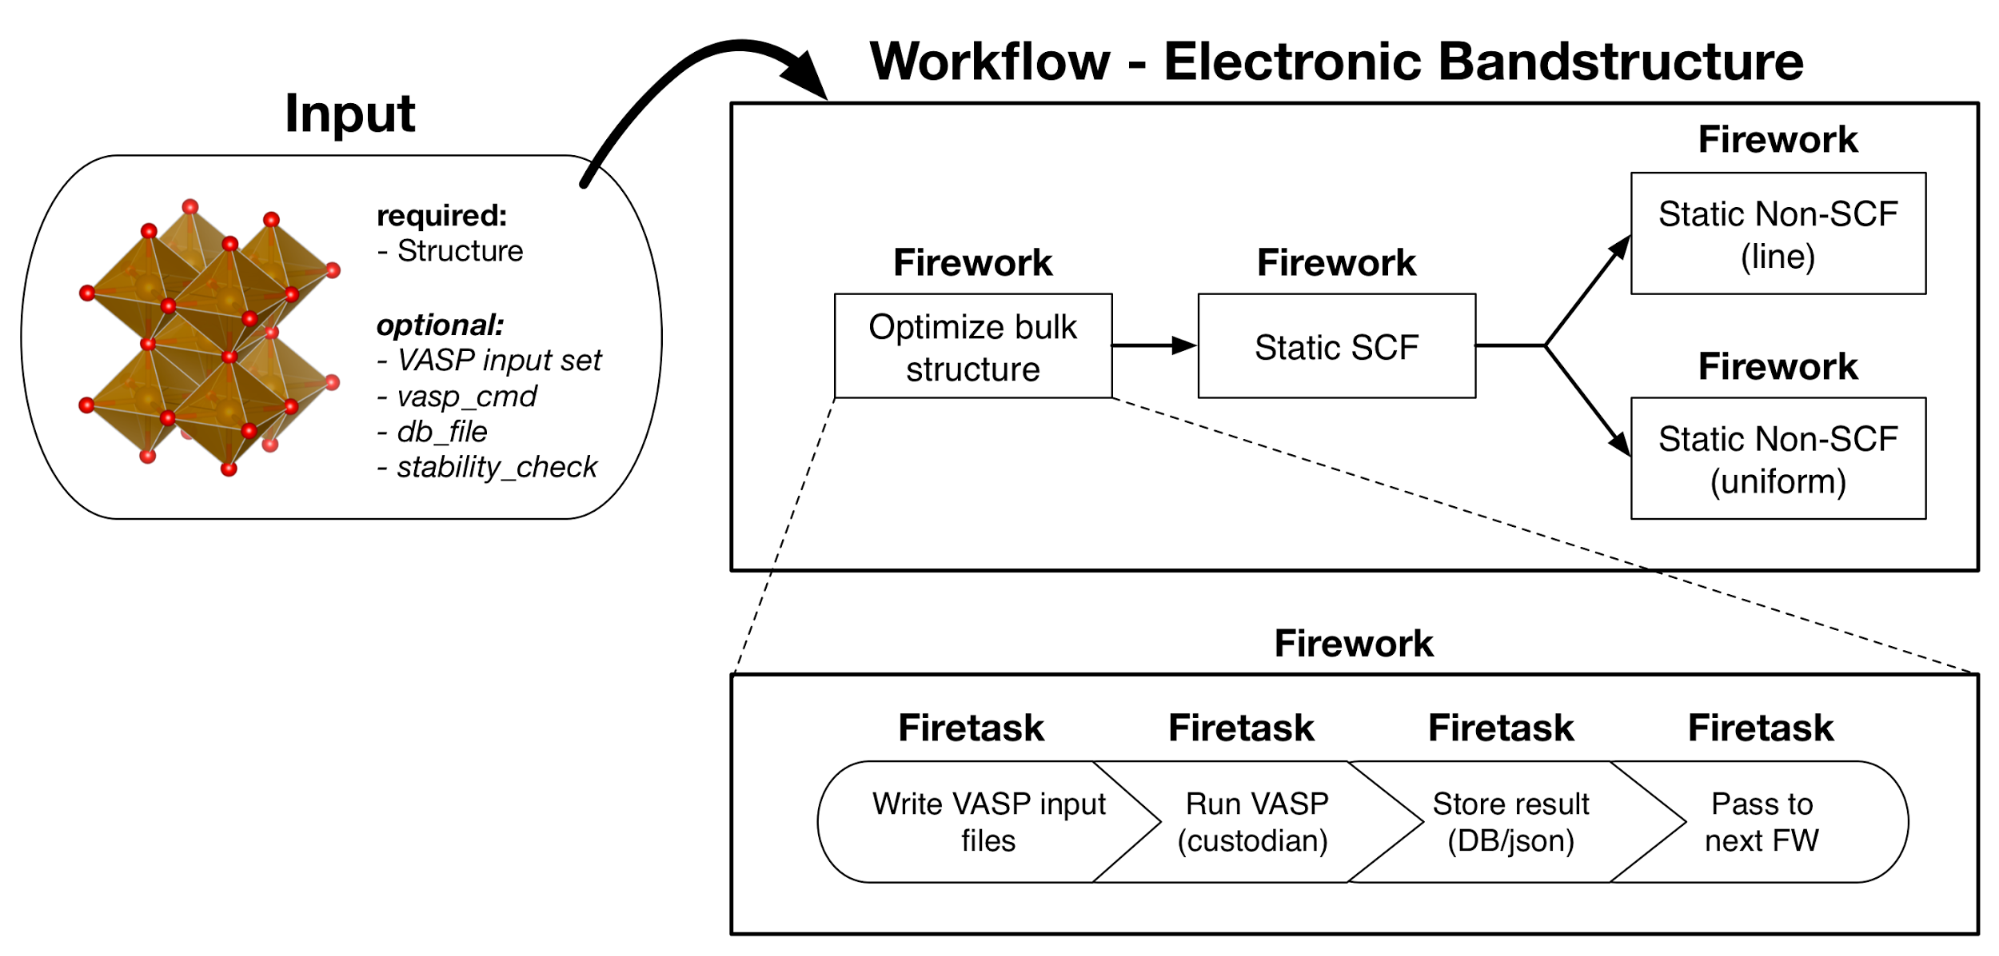
\includegraphics[height=1.5in]{Figures/bandstructure_wf.png}
%\caption{\fontsize{7.2pt}{4.2pt}\selectfont{\textrm{The integrated calculator in ASE (Atomic Simulation Environment).}}}%
\label{Logo_QM-MM}
\end{figure} 
}

\frame
{
	\frametitle{\textrm{ASE}自动流程的设计与管理}
		\textcolor{purple}{\textrm{ASE}}:~模块加载式计算流程控制,更符合复杂多尺度计算场景
		\begin{itemize}
			\item \textcolor{magenta}{灵活的建模功能}
				\begin{enumerate}
    \setlength{\itemsep}{10pt}
					\item 简单堆积:~原子直接组成分子
					\item 理想周期体系(包括一维、二维、三维)
					\item 表面和表面吸附,可指定吸附位
				\end{enumerate}
			\item \textcolor{magenta}{丰富的软件接口}\\
				提供了包括绝大部分第一原理和分子动力学计算软件接口,方便组合实现多尺度计算
			\item \textcolor{magenta}{不依赖软件的优化与动力学模拟}\\
				适合复杂材料物性模拟的优化和多种动力学过程模拟
			\item \textcolor{magenta}{多样化的数据库类型}
		\end{itemize} 
}

\frame
{
\frametitle{\textrm{ASE}特色:~材料结构生成模块}
\begin{figure}[h!]
\centering
\vspace*{-0.15in}
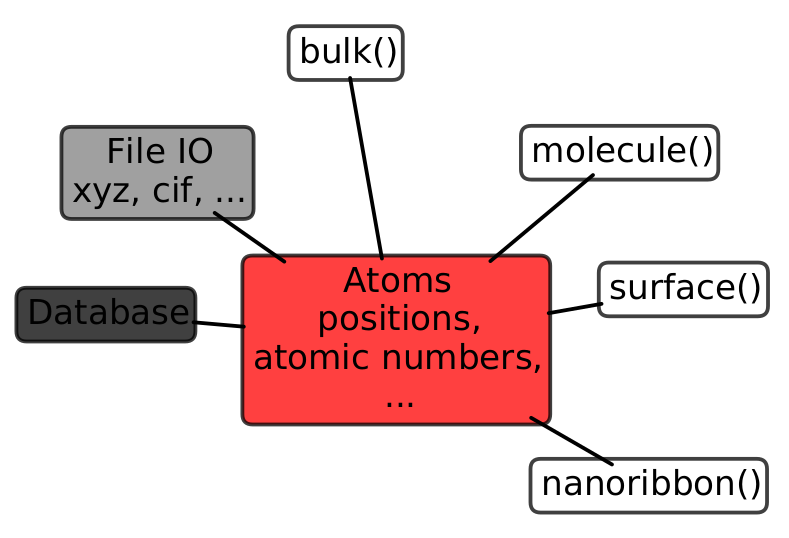
\includegraphics[height=1.2in,width=1.7in,viewport=0 0 820 530,clip]{Figures/ASE_atoms_module.png}
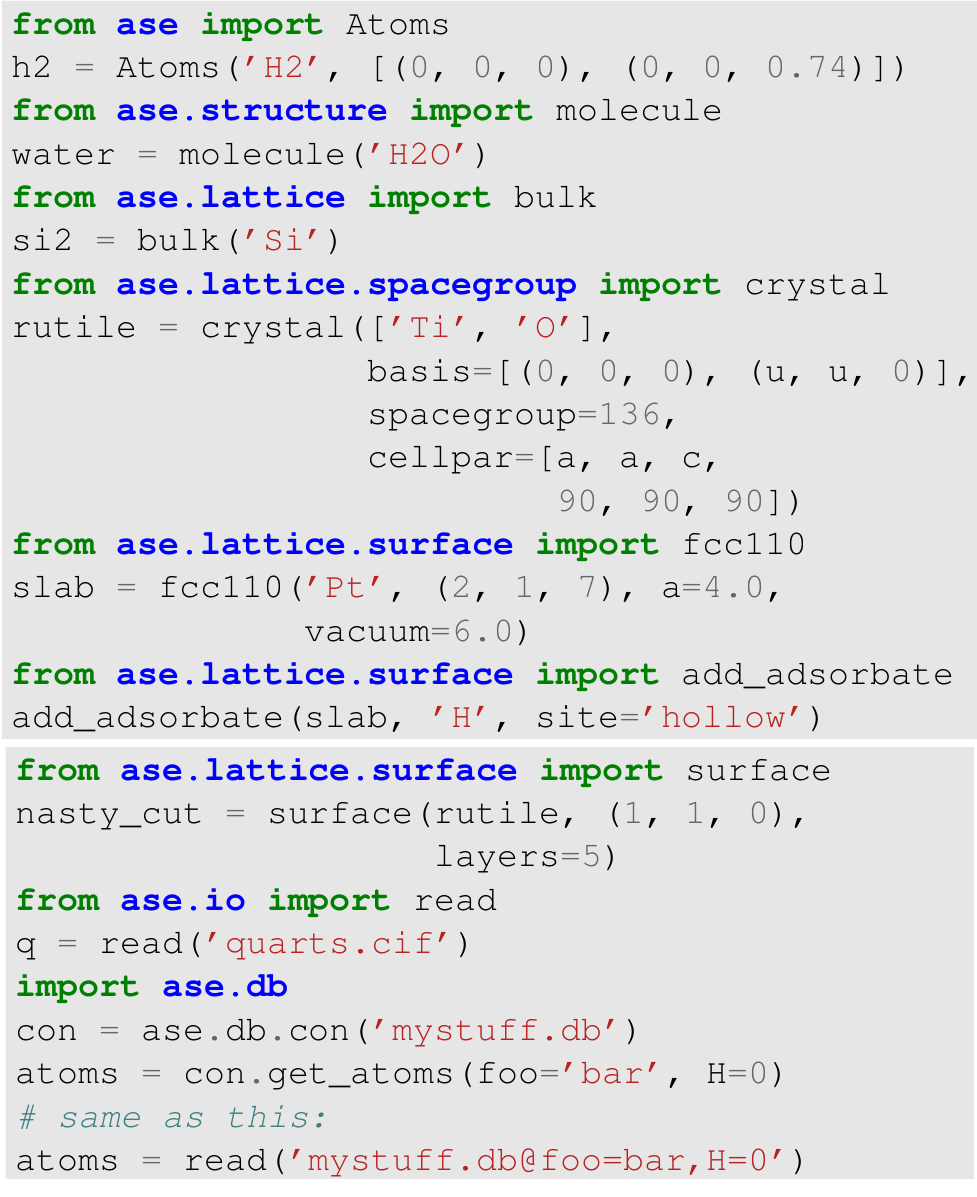
\includegraphics[height=2.9in,width=2.2in,viewport=0 0 970 1200,clip]{Figures/ASE_atoms_module-examples.png}
%\caption{\fontsize{7.2pt}{4.2pt}\selectfont{\textrm{The integrated calculator in ASE (Atomic Simulation Environment).}}}%
\label{Logo_atoms-module}
\end{figure} 
}

\frame
{
\frametitle{\textrm{ASE}特色:~软件接口丰富}
\textcolor{purple}{\textrm{ASE}}:~\textrm{Calculator}模块提供的可选的软件接口
\begin{figure}[h!]
\centering
\vspace*{-0.05in}
%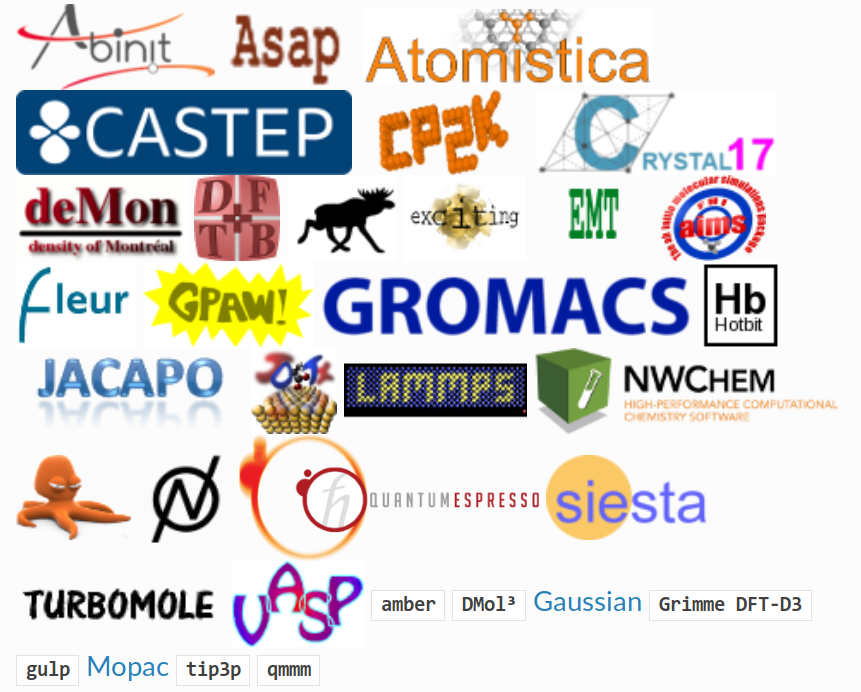
\includegraphics[height=1.0in,width=1.4in,viewport=0 0 638 530,clip]{Figures/ASE_calculator.png}
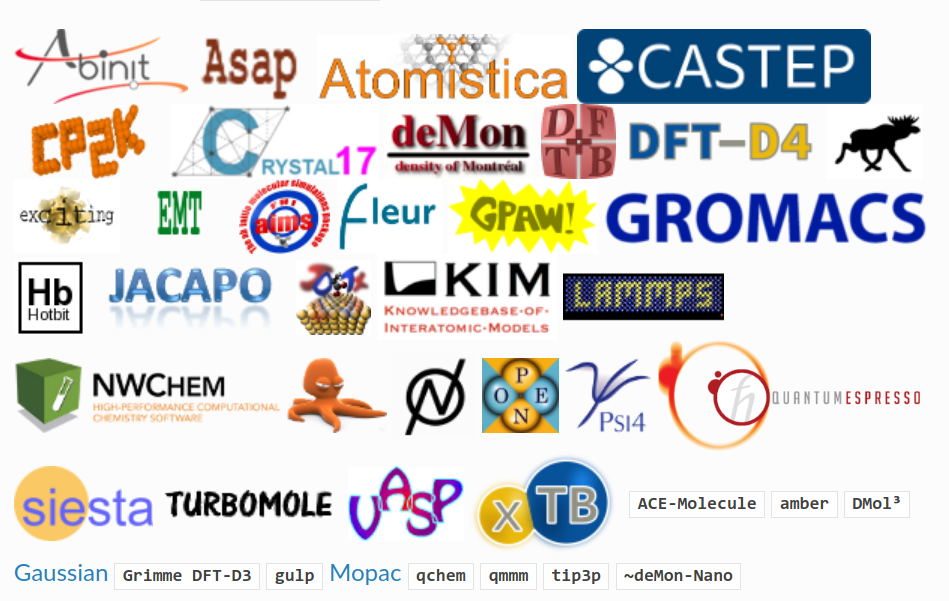
\includegraphics[height=2.0in,width=3.2in,viewport=0 0 940 600,clip]{Figures/ASE_calculator-new.png}
\caption{\fontsize{7.2pt}{4.2pt}\selectfont{\textrm{The integrated calculator in ASE.}}}%
\label{ASE_Calculator}
\end{figure} 
}

\frame
{
\frametitle{\textrm{ASE}特色:~提供多种优化算法模块和数据库}
\begin{figure}[h!]
\centering
\vspace*{-0.18in}
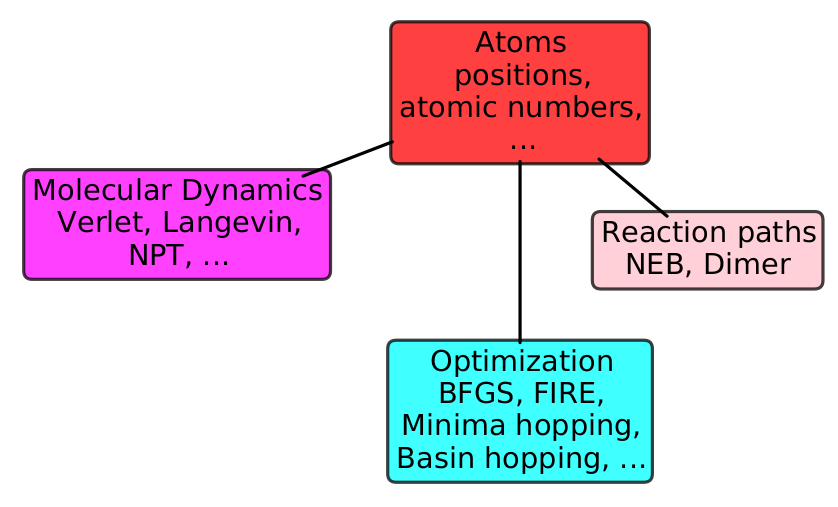
\includegraphics[height=1.3in,width=2.5in,viewport=0 0 838 500,clip]{Figures/ASE_opt_modules.png}
\vskip 1pt
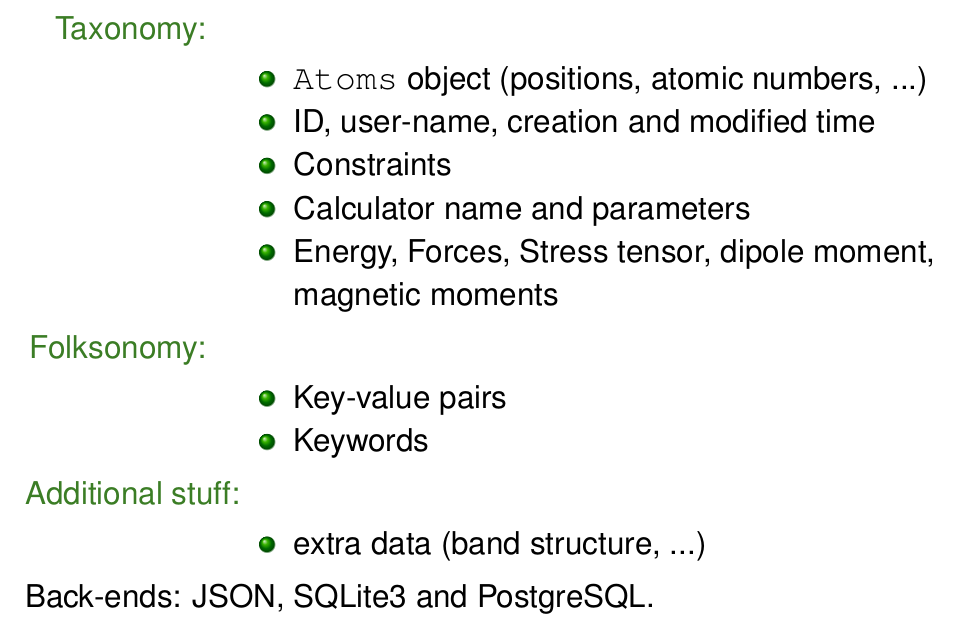
\includegraphics[height=1.7in,width=2.5in,viewport=0 0 938 630,clip]{Figures/ASE_database.png}
\label{ASE_opt-database}
\end{figure} 
}
%\frame
%{
%	\frametitle{\textrm{计算平台的作业自动提交:~基于\textrm{ASE}}}
%\begin{figure}[h!]
%\centering
%\vspace*{-0.2in}
%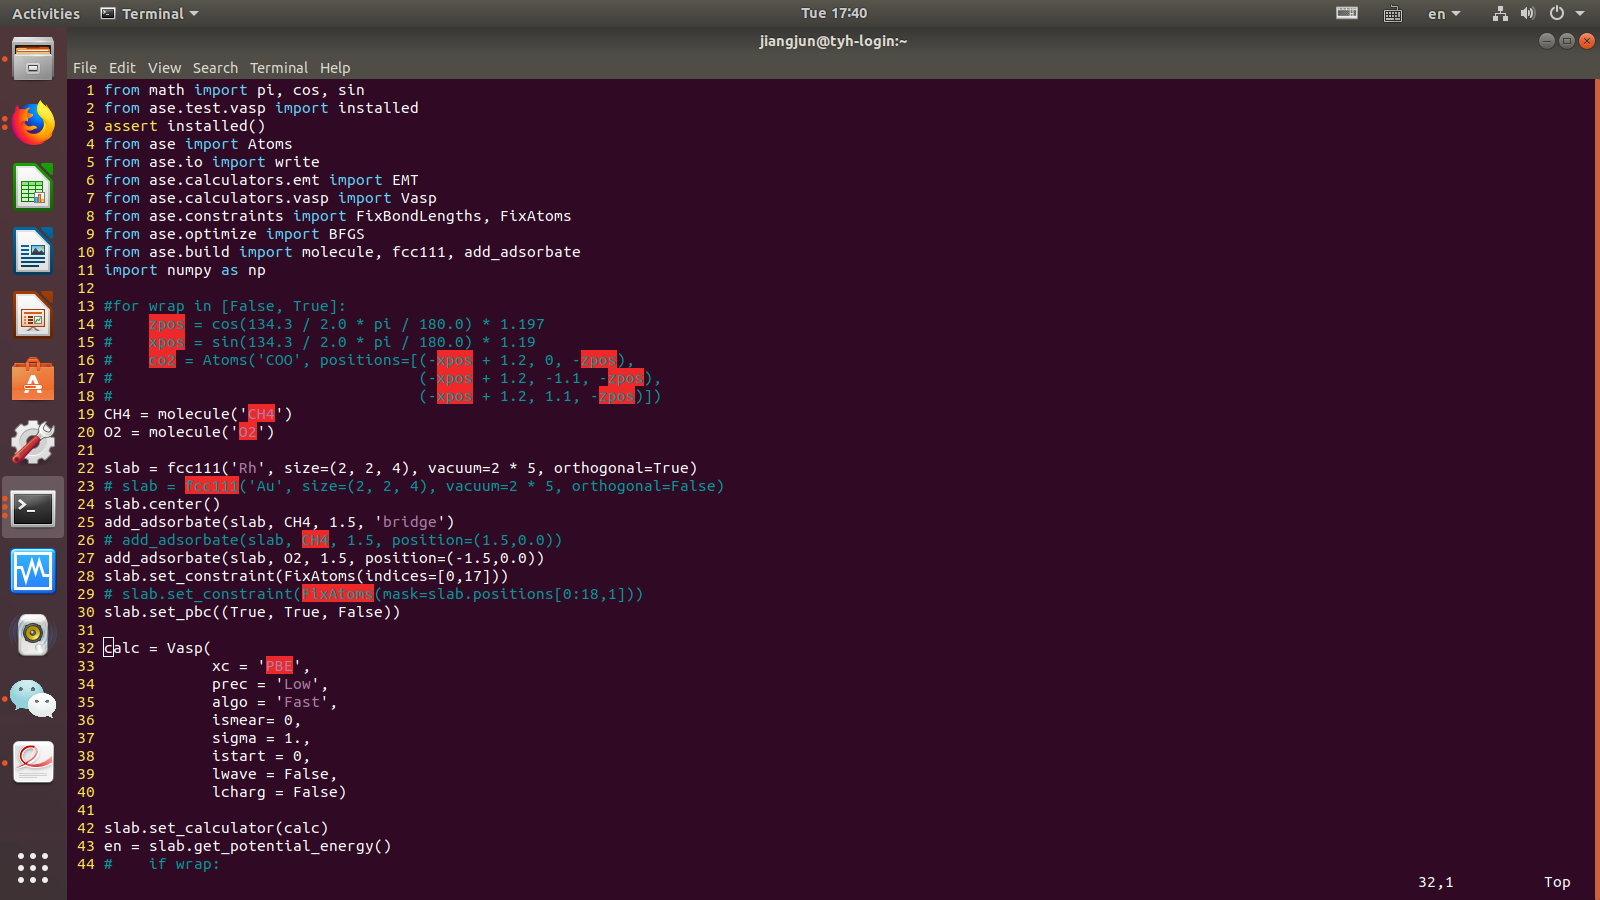
\includegraphics[height=3.1in,width=2.5in,viewport=75 0 725 820,clip]{Figures/ASE_app.png}
%%\caption{\fontsize{7.2pt}{4.2pt}\selectfont{\textrm{The integrated calculator in ASE (Atomic Simulation Environment).}}}%
%\label{ASE_app}
%\end{figure} 
%}

%\frame
%{
%	\frametitle{\textrm{计算平台的结果展示:~基于\textrm{MP}}}
%\begin{figure}[h!]
%\centering
%\vspace*{-0.2in}
%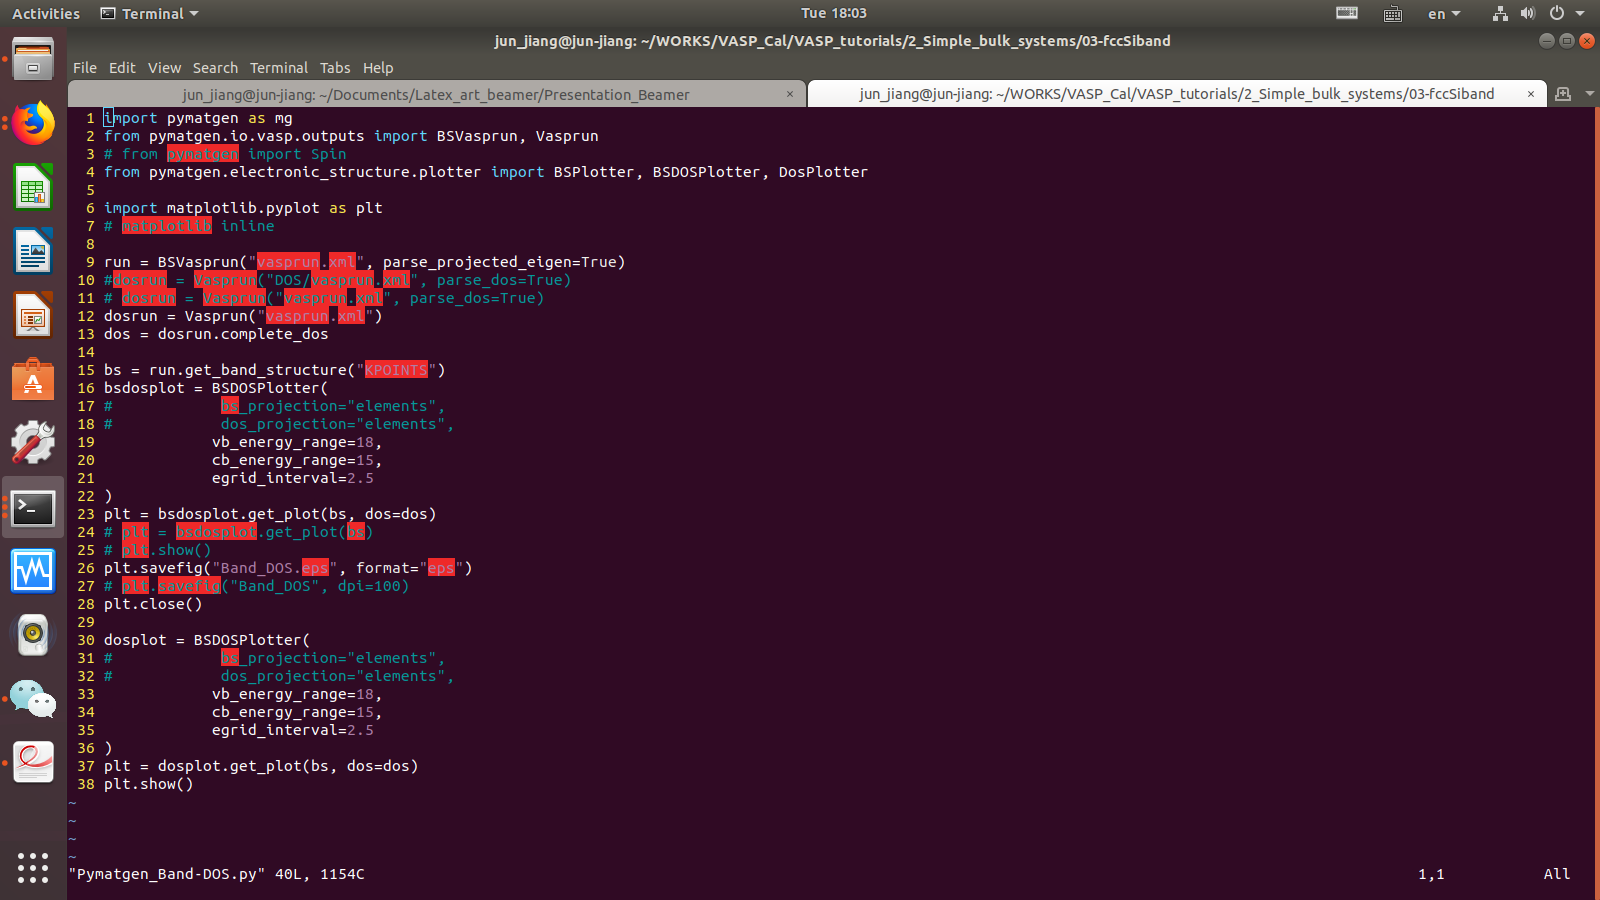
\includegraphics[height=3.1in,width=3.6in,viewport=73 80 880 790,clip]{Figures/Pymatgen_app.png}
%%\caption{\fontsize{7.2pt}{4.2pt}\selectfont{\textrm{The integrated calculator in ASE (Atomic Simulation Environment).}}}%
%\label{Pymatgen_app}
%\end{figure} 
%}
%
\frame
{
	\frametitle{\textrm{计算平台的结果展示:~结合\textrm{MP}与\textrm{ASE}}}
\begin{figure}[h!]
\centering
\vspace*{-0.2in}
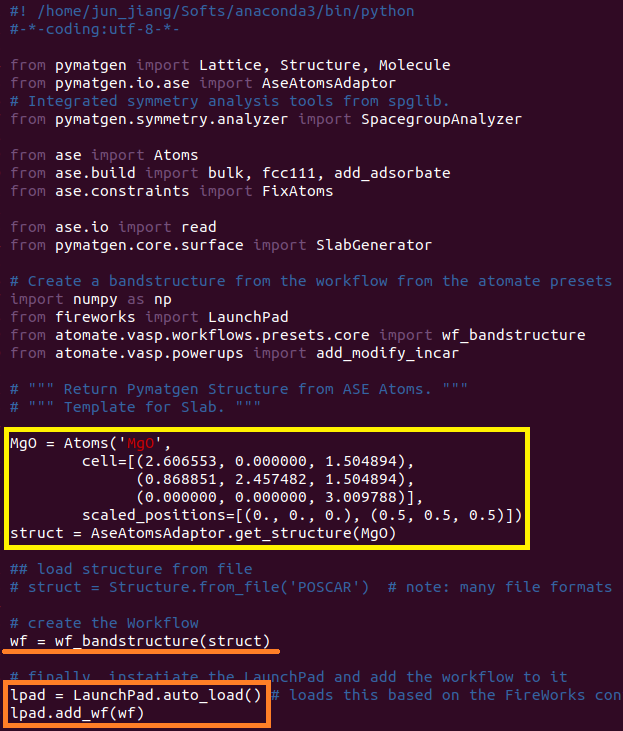
\includegraphics[height=3.0in,width=3.5in,viewport=0 0 600 550,clip]{Figures/Atomate-ASE_MgO.png}
%\caption{\fontsize{7.2pt}{4.2pt}\selectfont{\textrm{The integrated calculator in ASE (Atomic Simulation Environment).}}}%
\label{Atomate-ASE_app}
\end{figure} 
}

\frame
{
	\frametitle{应用示例:~\textrm{MgO:~DOS and Band}}
\begin{figure}[h!]
\centering
\vspace*{-0.16in}
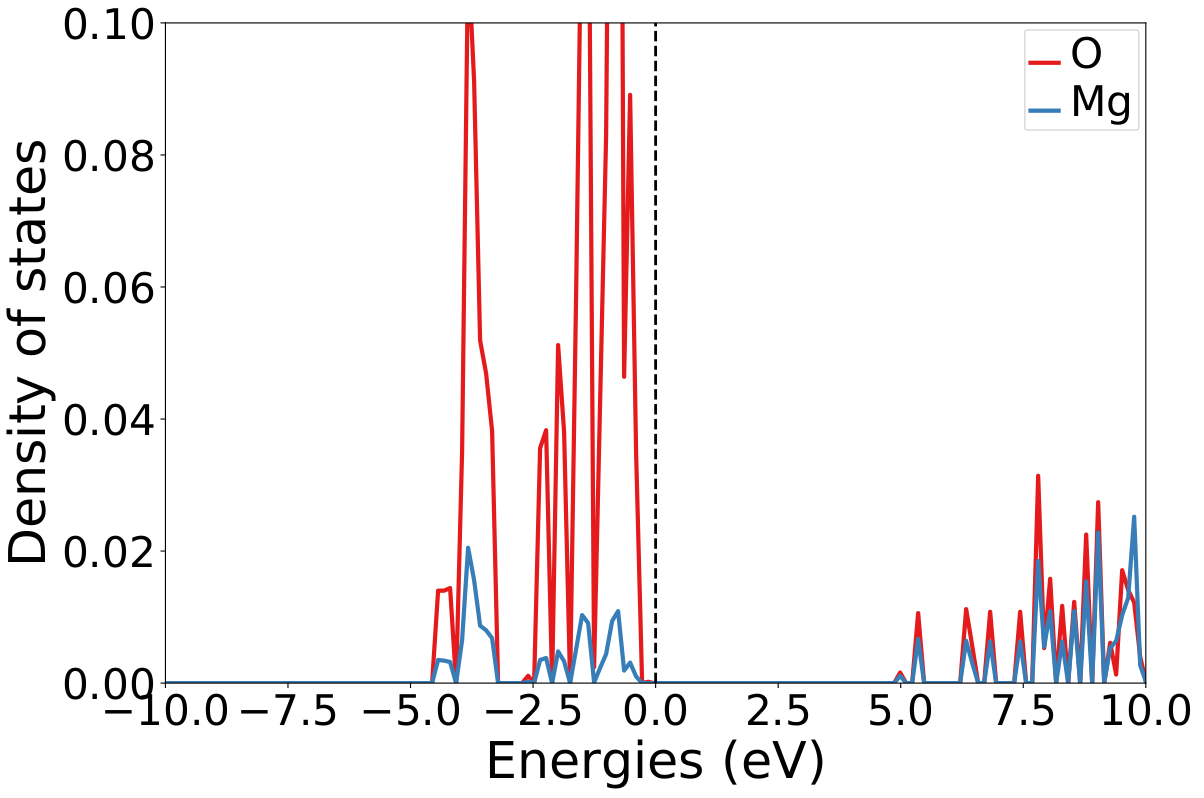
\includegraphics[height=1.5in,width=2.3in,viewport=0 0 900 600,clip]{Figures/Atomate_MgO-DOS.png}
\vskip 0.5pt
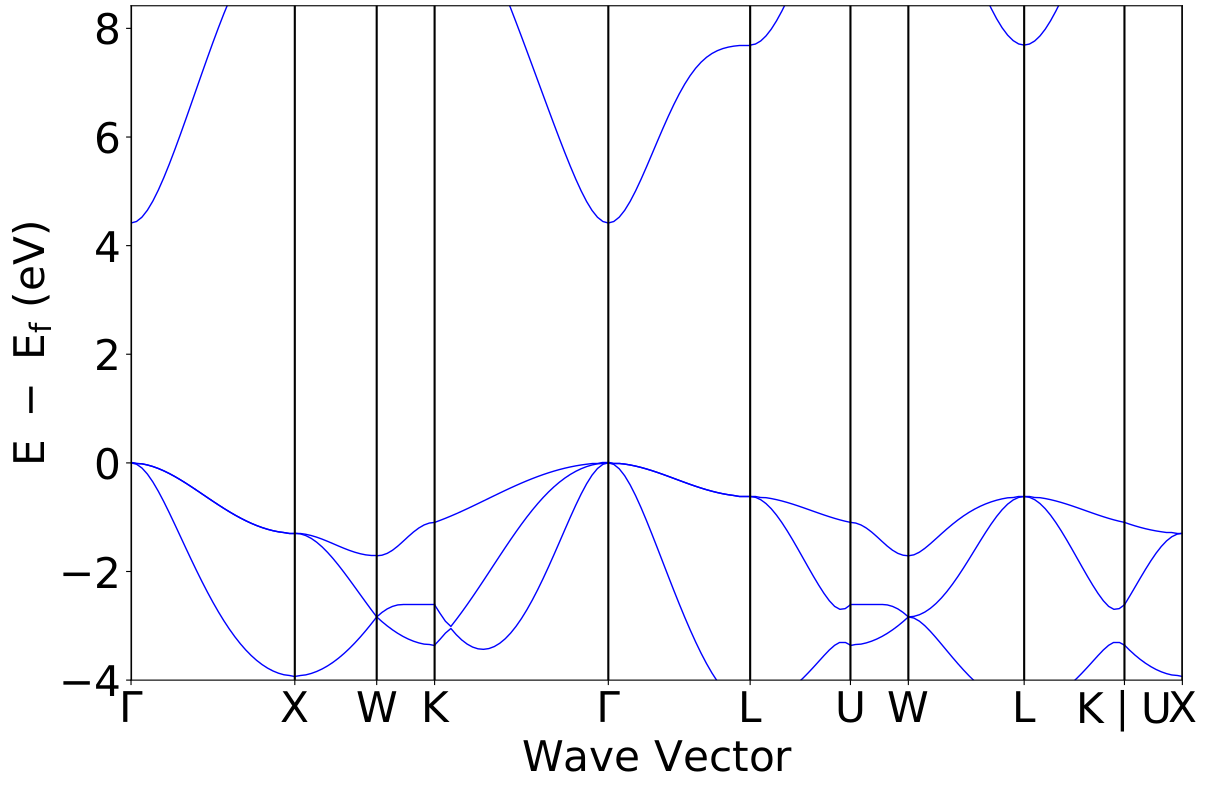
\includegraphics[height=1.5in,width=2.3in,viewport=0 0 900 600,clip]{Figures/Atomate_MgO-Band.png}
%\caption{\fontsize{7.2pt}{4.2pt}\selectfont{\textrm{The integrated calculator in Atomate-ASE.}}}%
\label{Atomate_MgO-DOS}
\end{figure} 
}

\section{\rm{VASP}计算的原子数据重建}
\frame
{
	\frametitle{\textrm{VASP}计算的原子数据基础}
	\textrm{POTCAR}提供了\textrm{VASP}计算所需的原子数据,也是实现\textrm{PAW}方法的主要基础
	\begin{itemize}
		\item \textrm{POTCAR}是\textrm{VASP}实现材料精确计算的重要保证\\
			同样都应用\textrm{PAW}方法,\textcolor{blue}{公认\textrm{VASP}较\textrm{QE}、\textrm{ABINIT}等软件的计算精度要高}
		\item \textrm{POTCAR}数据生成依赖较多的可调参数\\
			包括能量参数$\varepsilon_l$、多种截断半径$r_c$、$r_{\mathrm{vloc}}$、$r_{\mathrm{shape}}$、$r_{\mathrm{core}}$
		\item \textcolor{red}{\textrm{POTCAR}数据生成代码是\textrm{VASP}中唯一没有公开的}
		\item 用\textrm{VASP}模拟极端条件下材料物性的能力,受到\textrm{POTCAR}数据的制约
	\end{itemize}
	%文献\cite{PRB59-1758_1999}介绍了\textrm{POTCAR}的主要实现思想

当前研究主要尝试基于开源的\textrm{PAW}赝势生成软件(\textrm{atomPAW}),开发能生成\textrm{POTCAR}原子数据的功能
}

\frame
{
	\frametitle{\textrm{PAW}原子数据集:~\textrm{wave~function}}
	平滑赝原子分波函数
	\begin{displaymath}
		\tilde\phi_{i=Lk}(\vec r)=Y_L(\widehat{\vec r-\vec R})\tilde\phi_{lk}(|\vec r-\vec R|)
	\end{displaymath}
	根据\textrm{RRKJ}赝势构造的思想,赝分波函数由球\textrm{Bessel}函数线性组合%\upcite{JPCM6-8245_1994}
	\begin{displaymath}
		\tilde\phi_{lk}(r)=\left\{
		\begin{aligned}
			&\sum_{i=1}^2\alpha_ij_l(q_ir)\quad &r<r_c^l\\
			&\phi_{lk}(r)\quad&r>r_c^l
		\end{aligned}
		\right.
	\end{displaymath}
	调节系数$\alpha_i$和$q_i$赝分波函数$\phi_{lk}(r)$在截断半径$r_c^l$处两阶连续可微
%	投影子波函数$\tilde p_i$由\textrm{Gram-Schmidt}正交条件$\langle\tilde p_i|\tilde\phi_j\rangle=\delta_{ij}$确定
}

\frame
{
	\frametitle{\textrm{PAW}原子数据集:~\textrm{wave~function}}
\begin{figure}[h!]
\centering
\vskip -0.5in
\includegraphics[width=1.5in,height=2.7in,viewport=0 0 350 550, angle=-90, clip]{Figures/WAE-data.eps}
\vskip -0.2in
\includegraphics[height=2.7in,width=1.5in,viewport=0 0 350 550, angle=-90, clip]{Figures/WPS-data.eps}
\caption{\tiny \textrm{The partial wave function.}}%(与文献\cite{EPJB33-47_2003}图1对比)
\label{Wave_Function}
\end{figure}
}

\frame
{
	\frametitle{\textrm{PAW}原子数据集:~\textrm{core~density}}
	\textcolor{blue}{构造赝芯电荷密度$\tilde n_c$}:~在截断半径$r_{\mathrm{core}}$内的定义为
	$$\sum_{i=1,2}B_i\dfrac{\sin(q_ir)}r\quad r<r_{\mathrm{core}}$$
	调节系数$q_i$和$B_i$使得赝芯电荷密度$\tilde n_c(r)$在截断半径$r_{\mathrm{core}}$处的两阶导数连续
\begin{figure}[h!]
\vskip -0.5in
\centering
\hspace*{-0.1in}
\includegraphics[width=1.5in,height=2.35in,viewport=0 0 350 550, angle=-90, clip]{Figures/CORE-data.eps}
\hspace*{-0.7in}
\includegraphics[height=2.35in,width=1.5in,viewport=0 0 350 550, angle=-90, clip]{Figures/PCORE-data.eps}
\caption{\tiny \textrm{The core density.}}%(与文献\cite{EPJB33-47_2003}图1对比)
\label{core_density_Function}
\end{figure}
}

\frame
{
	\frametitle{\textrm{PAW}原子数据集:~$\mathrm{v}_{e\!f\!f}(r)$与$\tilde{\mathrm{v}}_{e\!f\!f}(r)$}
	\textcolor{blue}{原子局域有效势$\mathrm{v}_{e\!f\!f}^a$}
\begin{figure}[h!]
%\vskip -0.5in
\vskip -0.17in
\centering
%\includegraphics[width=1.6in,height=2.7in,viewport=0 0 300 460, angle=-90, clip]{Figures/POTAE-data.eps}
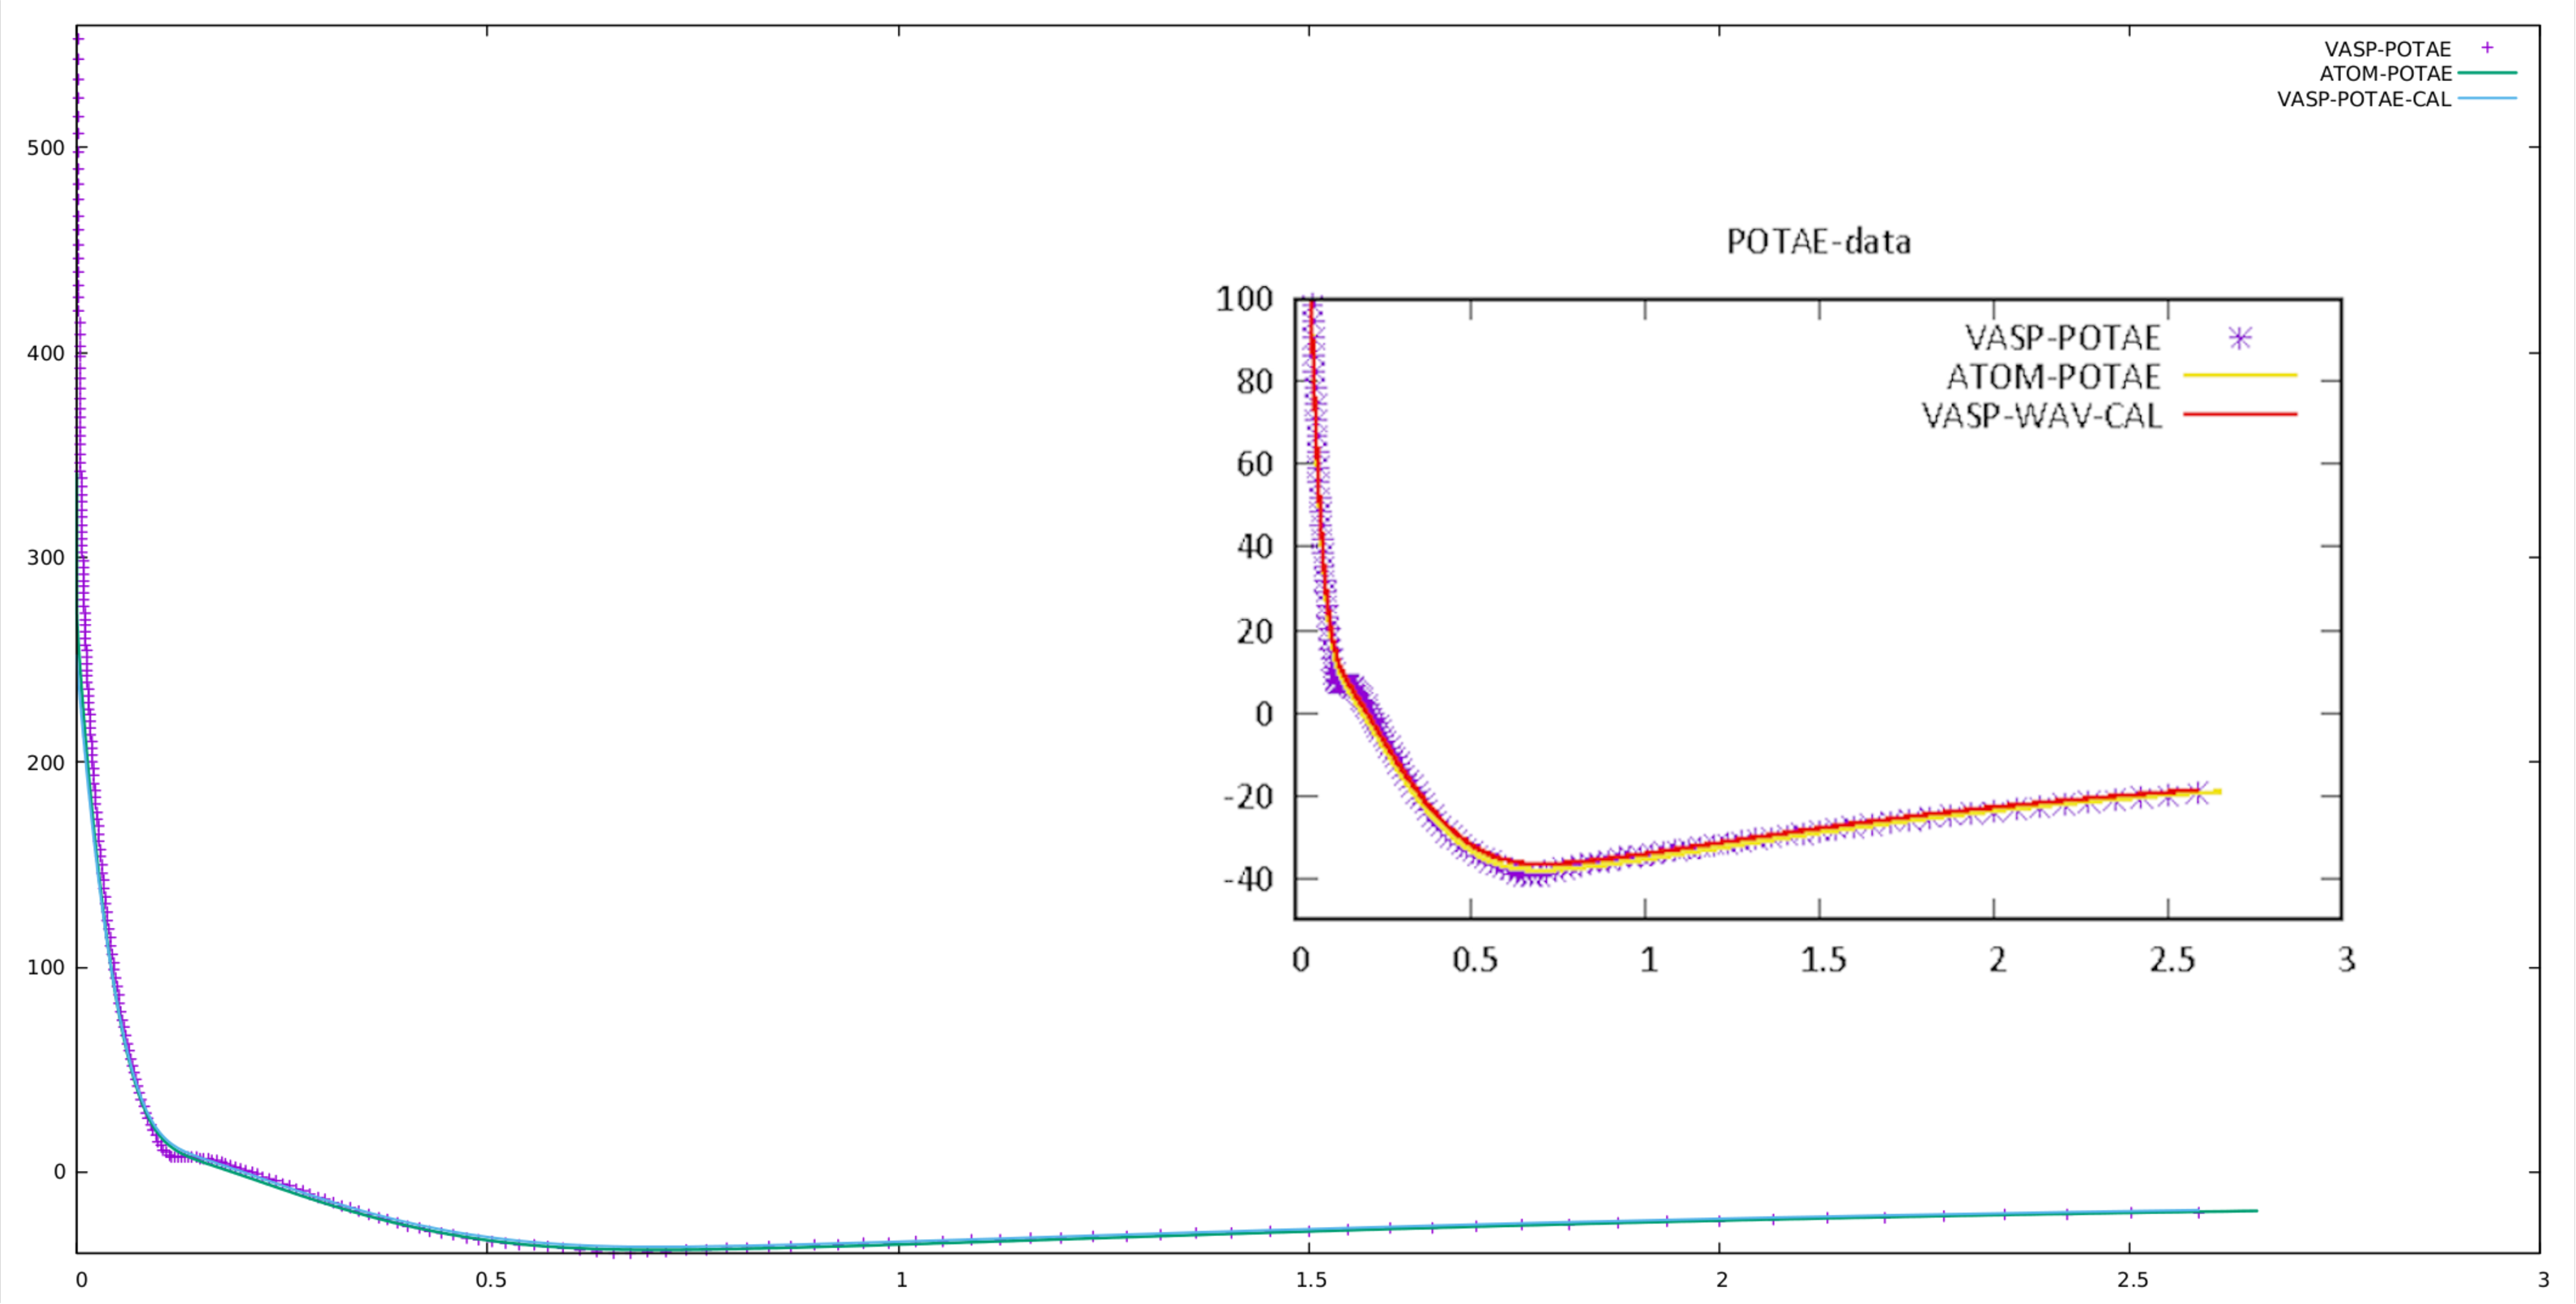
\includegraphics[width=2.5in,height=1.2in,viewport=0 0 1600 800, clip]{Figures/POTAE-full-dat.pdf}
\caption{\tiny \textrm{The local atomic effective-Potential.}}%(与文献\cite{EPJB33-47_2003}图1对比)
\label{local_atomic_PP}
\end{figure}
	\textcolor{blue}{构造原子局域赝势$\tilde v_{e\!f\!f}^a$}%(\textcolor{red}{为防止\textrm{ghost band}})
	:%\\
	(在截断半径$r_{\mathrm{loc}}$内的定义)
	$$\tilde v_{e\!f\!f}^a=A\dfrac{\sin(q_{loc}r)}r\quad r<r_{\mathrm{loc}}$$
	其中$q_{loc}$和$A$要求局域赝势在截断半径$r_{\mathrm{loc}}$处连续到一阶导数
}

\frame
{
	\frametitle{\textrm{PAW}原子数据集:~$\mathrm{v}_H[\tilde n_{Zc}]$}
	局域离子赝势$v_H[\tilde n_{Zc}]$可由原子局域赝势去屏蔽得到
	$$v_H[\tilde n_{Zc}]=\tilde v_{e\!f\!f}^a-v_H[\tilde n_a^1+\hat n_a]-v_{\mathrm{XC}}[\tilde n_a^1+\hat n_a+\tilde n_c]$$
\begin{figure}[h!]
\vskip -0.5in
\centering
\hspace*{-0.1in}
\includegraphics[width=1.5in,height=2.35in,viewport=0 0 350 550, angle=-90, clip]{Figures/POTPS-data.eps}
\hspace*{-0.7in}
\includegraphics[height=2.35in,width=1.5in,viewport=0 0 350 550, angle=-90, clip]{Figures/POTPSC-data.eps}
\caption{\tiny \textrm{The pseudo-potential and local ionic pseudo-potential.}}%(与文献\cite{EPJB33-47_2003}图1对比)
\label{pseudo_potential}
\end{figure}
}

\frame
{
	\frametitle{\textrm{VASP}计算的并行实现}
	\begin{itemize}
	     \item 中间层设计:~\textrm{FFT}网格、实空间基组与计算节点的匹配\\
		     \textcolor{red}{通过子程序\textrm{mgrid.F}生成中间层,实现并行负载与计算节点分配的匹配,减少\textrm{FFT}变换和实空间并行的节点间通信}
\begin{figure}[h!]
		\vspace{-0.25in}
	\centering
%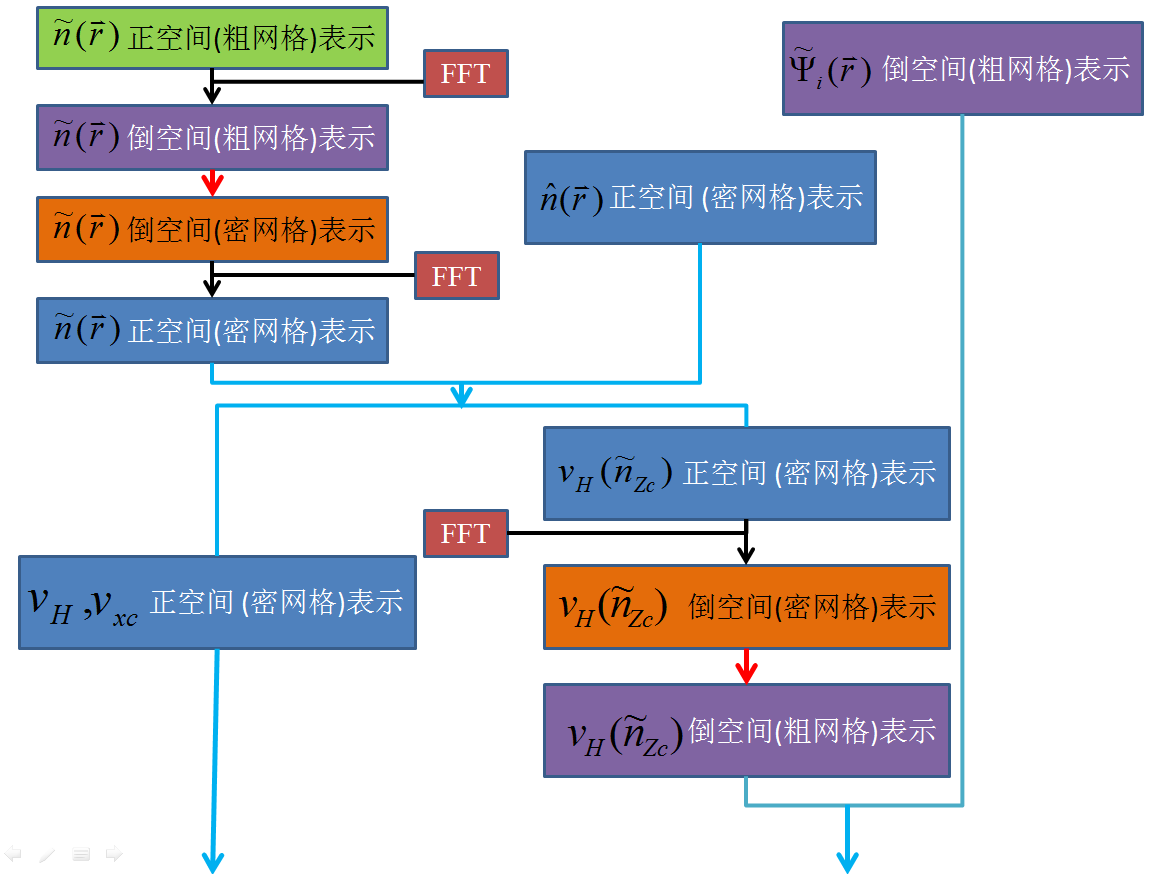
\includegraphics[height=2.7in,width=4.0in,viewport=0 0 1180 875,clip]{Figures/dual_grid.png}
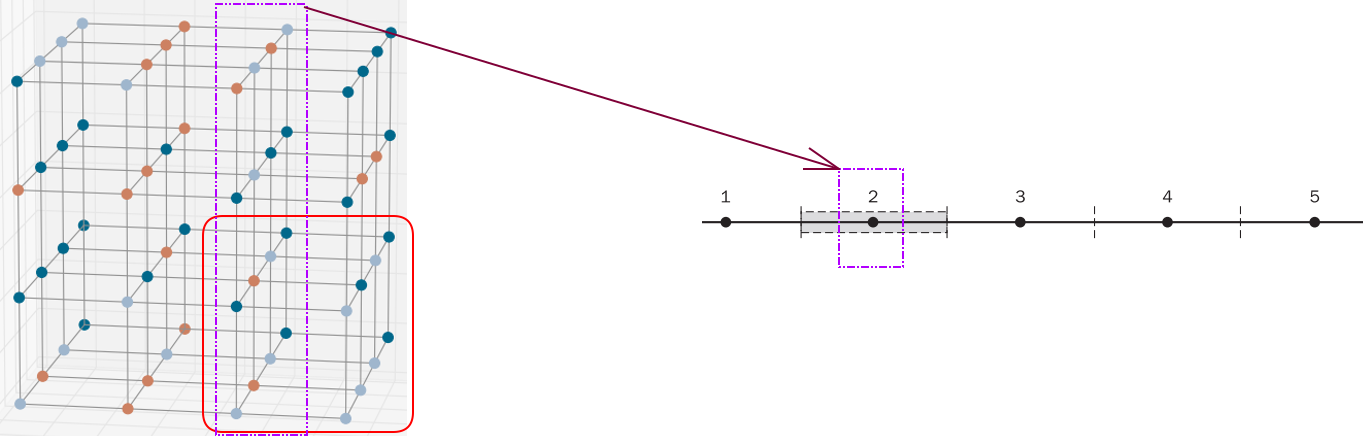
\includegraphics[height=1.0in,width=4.0in,viewport=0 0 1500 450,clip]{Figures/VASP_FFT-MPI_Reciprocal.png}
\vskip 0.5pt
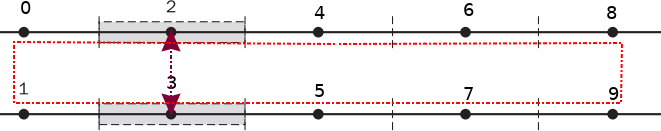
\includegraphics[height=0.7in,width=4.0in,viewport=0 0 730 150,clip]{Figures/VASP_FFT-MPI_Real.png}
\caption{\tiny \textrm{VASP:~ Reciprocal-Real space layout for grids in MPI.}}%(与文献\cite{EPJB33-47_2003}图1对比)
\label{MPI-FFT}
\end{figure} 
	\end{itemize}
}

%------------------------------------------------------------------------Reference----------------------------------------------------------------------------------------------
%\begin{thebibliography}{99}
%-----------------------------------------------------------------------------------------------------------------------------------------------------------------------%
%\frame
%{
%\frametitle{主要参考文献}
%{\small
%\bibitem{Singh_Book}\textrm{D. J. Singh. \textit{Plane Wave, PseudoPotential and the LAPW method} (Kluwer Academic, Boston,USA, 1994)}					%
%  \nocite{*}																				%
%}
%}
%\end{thebibliography}
